\chapter{Hello World}

\section{Introduzione}
In questo capitolo applicheremo i concetti teorici descritti precedentemente per sviluppare un software basato sui microservizi. Lo scopo è quello di verificare come tale approccio permette uno sviluppo più semplice delle applicazioni dividendo l'intera logica di business in piccoli servizi ognuno indipendente dall'altro.


\subsection{Pom di Spring Boot}
L'utilizzo di Spring Boot come framwork back-end genera un file pom con delle informazioni di base. Queste informazioni sono condivise tra tutti i progetti che utilizzano Maven e Spring Boot.

\begin{lstlisting}[language=XML]
	<!-- ... -->
	<parent>
		<groupId>org.springframework.boot</groupId>
		<artifactId>spring-boot-starter-parent</artifactId>
		<version>2.7.5</version>
		<relativePath/> <!-- lookup parent from repository -->
	</parent>
	<!-- ... -->
			<plugin>
				<groupId>org.springframework.boot</groupId>
				<artifactId>spring-boot-maven-plugin</artifactId>
			</plugin>

\end{lstlisting}

Nel nostro caso l'estratto del pom riportato indica l'aggiunta dell'utilizzo del framwork Spring Boot alla versione 2.7.5 e l'aggiunta del plugin ufficiale sviluppato da Spring Boot.


\subsection{Struttura dei servizi}
Per la gestione dei singoli progetti abbiamo utilizzato Apache Maven. Come spiegato nei precedenti capitoli, Maven è un ottimo strumento, non solo permette di soddisfare tutte le dipendenze richieste dall'applicativo, ma permette anche di standardizzare la struttura di un progetto, per Spring Boot la struttura è molto simile ad un semplice progetto in Java. 


\begin{figure}[h!]
    \centering
    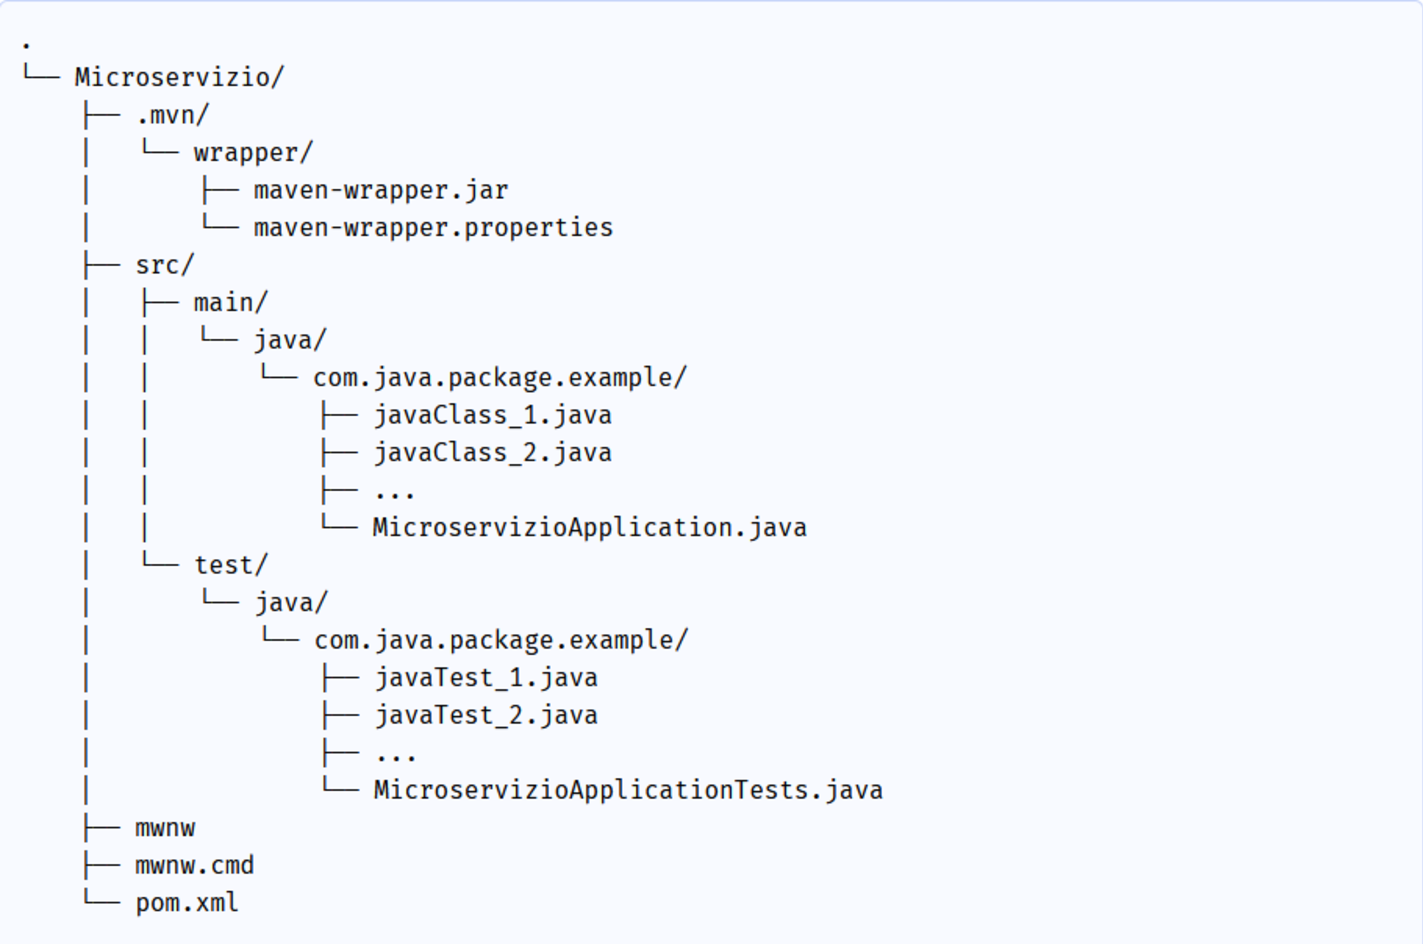
\includegraphics[scale = 0.60]{capitoli/immagini/11_maven_tree.pdf}
    \caption{Struttura per i progetti in Spring Boot}
    \label{fig:maven_structure_springboot}
\end{figure}

\section{Architettura}

L'applicazione sviluppata presenta tutta la logica di business all'interno di due microservizi. Image Service è il primo servizio sviluppato, il suo scopo è quello di recuperare delle informazioni su delle immagini. Gallery Service invece ha il compito di filtrare le varie immagini esposte dal servizio precedentemente elencato.

\begin{figure}[h]
    \centering
    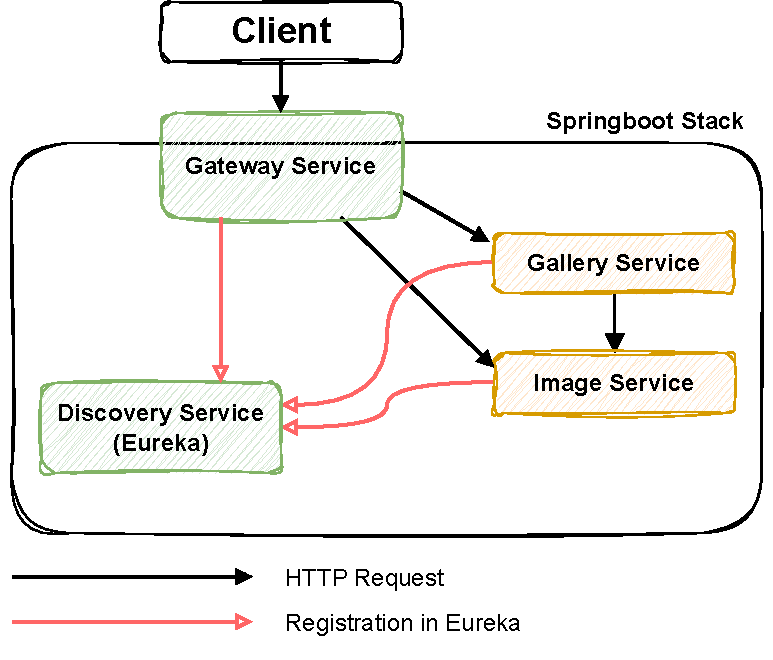
\includegraphics[scale = 0.65]{capitoli/immagini/12_architettura_hello_world.pdf}
    \caption{Architettura del software}
    \label{fig:architettura_hello_worlds}
\end{figure}

Come possiamo notare dal diagramma dell'architettura, sono riportati altri due servizi che prima non sono stati menzionati. Il gateway service ha l'obiettivo di esporre l'intera applicazione all'utente finale tramite un singolo punto di accesso. L'utente digitando l'\ac{URL} esposto dal servizio di gateway nel proprio browser, riesce ad accedere immediatamente all'applicazione, ma in realtà sarà il gateway che si occuperà di instradare i dati in entrata e in uscita.

Il discovery service è forse il più importante perché permette di gestire tutti i servizi che compongono l'applicazione, anche quelli non visibili all'utente finale. Eureka è il nome del discovery service messo a disposizione dal framework Spring Boot.




\subsection{Eureka Discovery Service}
Il servizio di scoperta si occupa di registrare tutti i servizi dell'applicazione in modo da poter esser gestiti. 

\paragraph{File di configurazione}
Il file di configurazione per i progetti che utilizzano il framework Spring Boot è denominato application.properties \footnote{In alcuni vecchi progetti o nella documentazione ufficiale è possibile trovare questo file con l'estensione yaml}. All'interno sono specificati parametri che aiutano la configurazione delle applicazioni. Nel caso del nostro servizio il file in questione è scritto in questo modo:

\begin{lstlisting}[caption=Application.properties di Eureka]
spring.application.name=eureka-server

server.port=8761

eureka.instance.prefer-ip-address=true
eureka.client.register-with-eureka=false
eureka.client.fetch-registry=false
\end{lstlisting}

Nel file sono riportate alcune informazioni base come il nome e la porta su cui verrà esposto il servizio, questo parametro andrà a sovrascrivere la configurazione base del server Tomcat che di default espone gli applicativi sulla porta 8080. dato che la nostra applicazione avrà diverse componenti conviene assegnare ad ognuno una porta diversa.

Ulteriori informazioni impostano dei parametri per il servizio eureka, in questo file specifichiamo che diamo libero arbitrio ad Eureka per quando riguarda la gestione della registrazione dell'indirizzo ip dei vari microservizi.

L'implementazione di Eureka prevede la presenza di due enti, il server e i client. Il servizio di discovery si comporta da server mentre i vari microservizi da client, quest'ultimi una volta effettuato il deploay cercheranno subito di contattare il discovery service (server) per effettuare la registrazione.

\paragraph{Gestione dei servizi}
Spring Boot espone un endpoint per il servizio Eureka che permette di accedere ad una dashboard per verificare lo stato dell'intero sistema, compresi i servizi che sono riusciti a registrarsi ad Eureka

\begin{figure}[h]
    \centering
    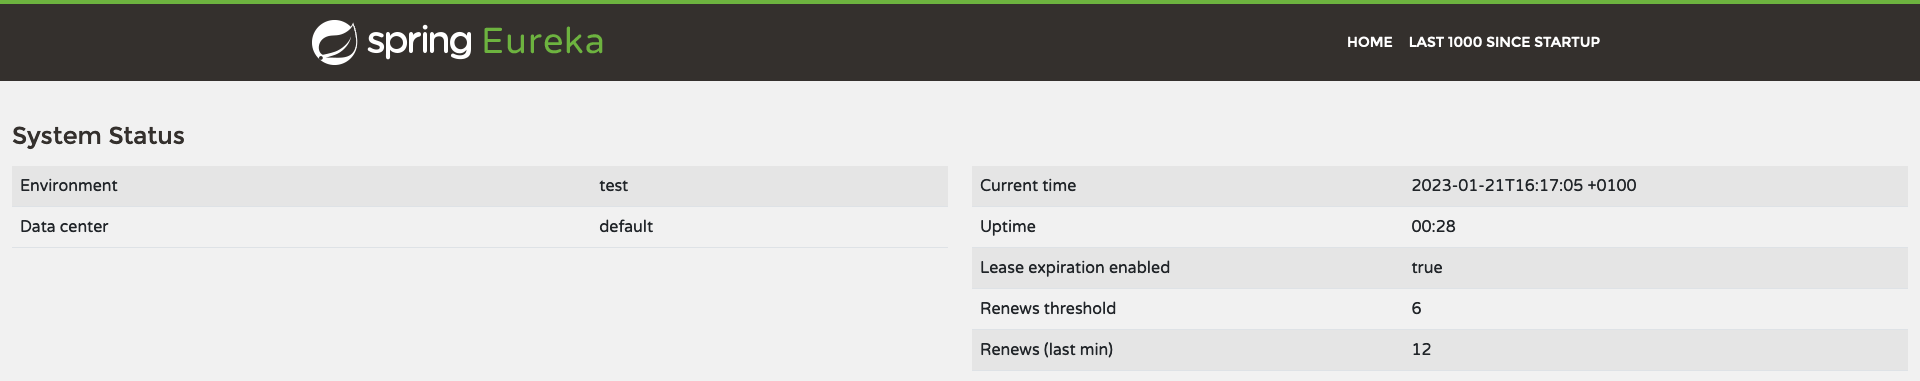
\includegraphics[scale=0.20]{capitoli/immagini/13_general_info.png}
    \caption{Informazioni generali sul servizio Eureka}
    \label{fig:General_info}
\end{figure}

Nella stessa pagina possibile non solo verificare lo stato del discovery service, ma anche i servizi registrati, il loro stato e il loro indirizzo di registrazione locale in tempo reale.

\begin{figure}[h]
    \centering
    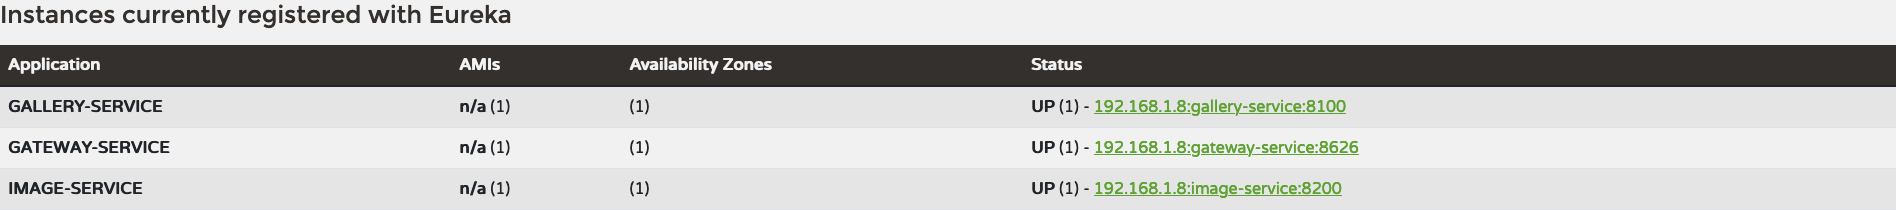
\includegraphics[scale=0.20]{capitoli/immagini/14_subscribe_services.png}
    \caption{Informazioni sui microservizi sottoscritti ad Eureka}
    \label{fig:Subscribe_Services}
\end{figure}

\subsection{Gateway Service}
Spring Cloud Gateway \cite{gateway} ha l'obiettivo di fornire un meccanismo di instradamento ai servizi che permetta di mantenere aspetti come la sicurezza e il monitoraggio delle risorse.

\begin{figure}[h]
    \centering
    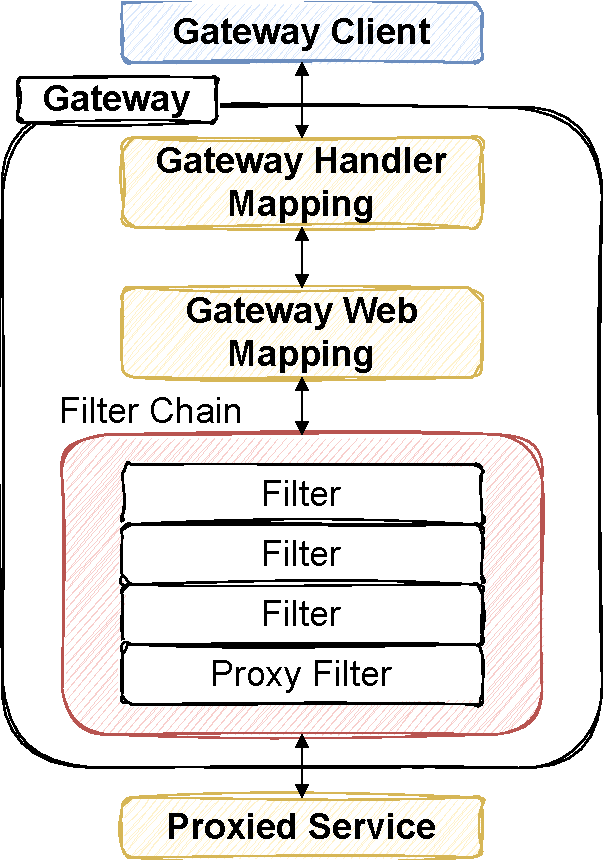
\includegraphics[scale=0.65]{capitoli/immagini/15_gateway_work.pdf}
    \caption{Funzionamento di Spring Cloud Gateway}
    \label{fig:gateway_work}
\end{figure}

Quando il servizio riceve una richiesta da un client, il componente Gateway Handler Mapping si occupa di riconoscere se il percorso inserito è corretto, in caso affermativo invia la richiesta al Gateway Web Handler che gestisce la richiesta, quest'ultima passa attraverso ad una serie di filtri che implementano logica di sicurezza, ed infine si collega al servizio richiesto dal client.

Durante la configurazione di tale servizio è necessario specificare i vari percorsi dei servizi. Nel nostro caso dobbiamo specificare due servizi, Image Service e Gallery Service, in questo modo il gateway sarà instruito su come instradare il traffico dei dati. Nel file application.properties specifichiamo tre attributi principali:

\begin{lstlisting}[caption=Application.properties del Gateway]
spring.cloud.gateway.routes[0].id=gallery
spring.cloud.gateway.routes[0].uri=lb://GALLERY-SERVICE
spring.cloud.gateway.routes[0].predicates[0]=Path=/gallery/**

spring.cloud.gateway.routes[1].id=image
spring.cloud.gateway.routes[1].uri=lb://IMAGE-SERVICE
spring.cloud.gateway.routes[1].predicates[0]=Path=/image/**
\end{lstlisting}

Possiamo notare che gli URI presenti nella configurazione coincidono con i nomi dei servizi che sono registrati sul server eureka \ref{fig:General_info}, questo perché il Gateway andrà a ricercare questi servizi proprio nel server di Eureka, nel caso i nomi non coincida quando si andrà a richiedere al Gateway di instradare del traffico verso un servizio quest'ultimo restituirà una pagina di errore.

Sempre nell'URI è possibile osservare che prima di ogni nome di servizio compare "lb", il gateway oltre all'instradamento del traffico si occupa anche di applicare una politica di load balancer, in modo da poter gestire il carico di lavoro in entrata e in uscita.


\begin{comment}
\subsection{Image Service - Logica di Business}

\begin{lstlisting}[language=Java]
@RestController
@RequestMapping(path = "/image")
public class HomeController {
    @Autowired
    private Environment env;
    @RequestMapping
    public String Home() {
        return "Hello from Image Service runnig at port: " + env.getProperty("local.server.port");
    }
    @RequestMapping(path = "/all")
    public List<Image> getImages() {
        return Arrays.asList(
                new Image(1, 
                        "Treehouse of Horror V", 
                        "https://www.imdb.com/title/tt0096697/mediaviewer/rm3842005760"),
                new Image(2, 
                        "The Town", 
                        "https://www.imdb.com/title/tt0096697/mediaviewer/rm3698134272"),
                new Image(3, 
                        "The Last Traction Hero", 
                        "https://www.imdb.com/title/tt0096697/mediaviewer/rm1445594112"));
    }
}
\end{lstlisting}

\subsection{Gallery Service - Logica di Business}

\begin{lstlisting}[language=Java]

@RestController
@RequestMapping(path = "/gallery")
public class HomeController {

    @Autowired
    private RestTemplate restTemplate;

    @Autowired
    private Environment env;

    @RequestMapping
    public String Home() {
        return "Hello from Gallery Service runnig at port: " + env.getProperty("local.server.port");
    }
    @RequestMapping(path = "/{id}")
    public Gallery getGallery(@PathVariable final int id){
        Gallery gallery = new Gallery();
        gallery.setId(id);

        List<Object> images = restTemplate.getForObject("http://image-service/image/all", List.class);
        gallery.setImages(images);

        return gallery;
    }
    @RequestMapping(path = "/admin")
    public String homeAdmin(){
        return "this is the admin area of Gallery Service running at port: " + env.getProperty("local.server.port");
    }
}

\end{lstlisting}
\end{comment}

\subsection{Avvio dei servizi}
L'ordine di deploy dei servizi è importante, il discovery service deve essere il primo servizio ad essere disponibile questo perché i vari servizi appena avviati invieranno una richiesta di registrazione e se Eureka è offline i servizi si arresteranno con un errore. L'ordine utilizzato per l'avvio dell'applicativo è il seguente:

\begin{enumerate}
    \item Eureka Server Service;
    \item Image Service;
    \item Gallery Service;
    \item Gateway Service;
\end{enumerate}

L'ordine di avvio del gateway non è importante, il servizio in questione effettuerà periodicamente una chiamata ad Eureka per verificare la presenza di nuovi servizi, se presenti verificherà il nome di quest'ultimi con i nomi specificati nel proprio file di configurazione.

\section{Aggiunta di un nuovo servizio}
Abbiamo detto più volte che grazie all'approccio ai microservizi andiamo a creare un software modulare con i servizi che sono indipendenti gli uni dagli altri, questo ci dice che è anche possibile implementare nuove tecnologie molto più facilmente.

\subsection{World Service}
World è il risultato del lavoro svolto durante l'attività di tirocinio presso Kineton. Sviluppato con Spring Boot, tale servizio si basa sul database world, una banca dati messa a disposizione gratuitamente dal sito di MySQL. Per prima cosa andiamo a modificare il diagramma dell'architettura visto precedentemente per implementare questo nuovo servizio:

\begin{figure}[h]
    \centering
    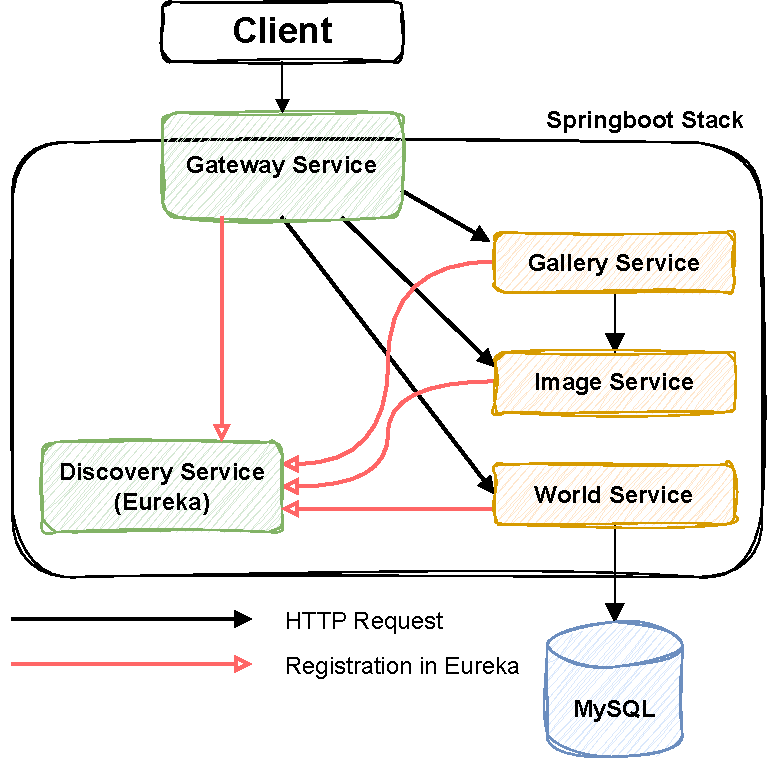
\includegraphics[scale=0.65]{capitoli/immagini/16_architettura_world.pdf}
    \caption{Architettura modificata con l'aggiunta di World Service}
    \label{fig:new_architecture}
\end{figure}

Oltre ad aver inserito il servizio che si occupa di esporre le API facciamo anche affidamento su un database che contiene i nostri dati.

\paragraph{Diagramma Entità Relazione di World}
Il diagramma ER del database World è formato da tre tabelle. Le due tabelle countrylanguage e city sono in relazione con la tabella country tramite una relazione uno a molti.
Nella tabella countrylanguage, l'attributo Language è una chiave primaria per la tabella e l'attributo countryCode è dichiarata come chiave primaria e come chiave esterna che fa riferimento al'attributo Code di country. Anche nella tabella city l'attributo CountryCode è una chiave esterna, che fa riferimento all'attributo Code di country. Infine in country la chiave primaria è Code.

\begin{figure}[h]
    \centering
    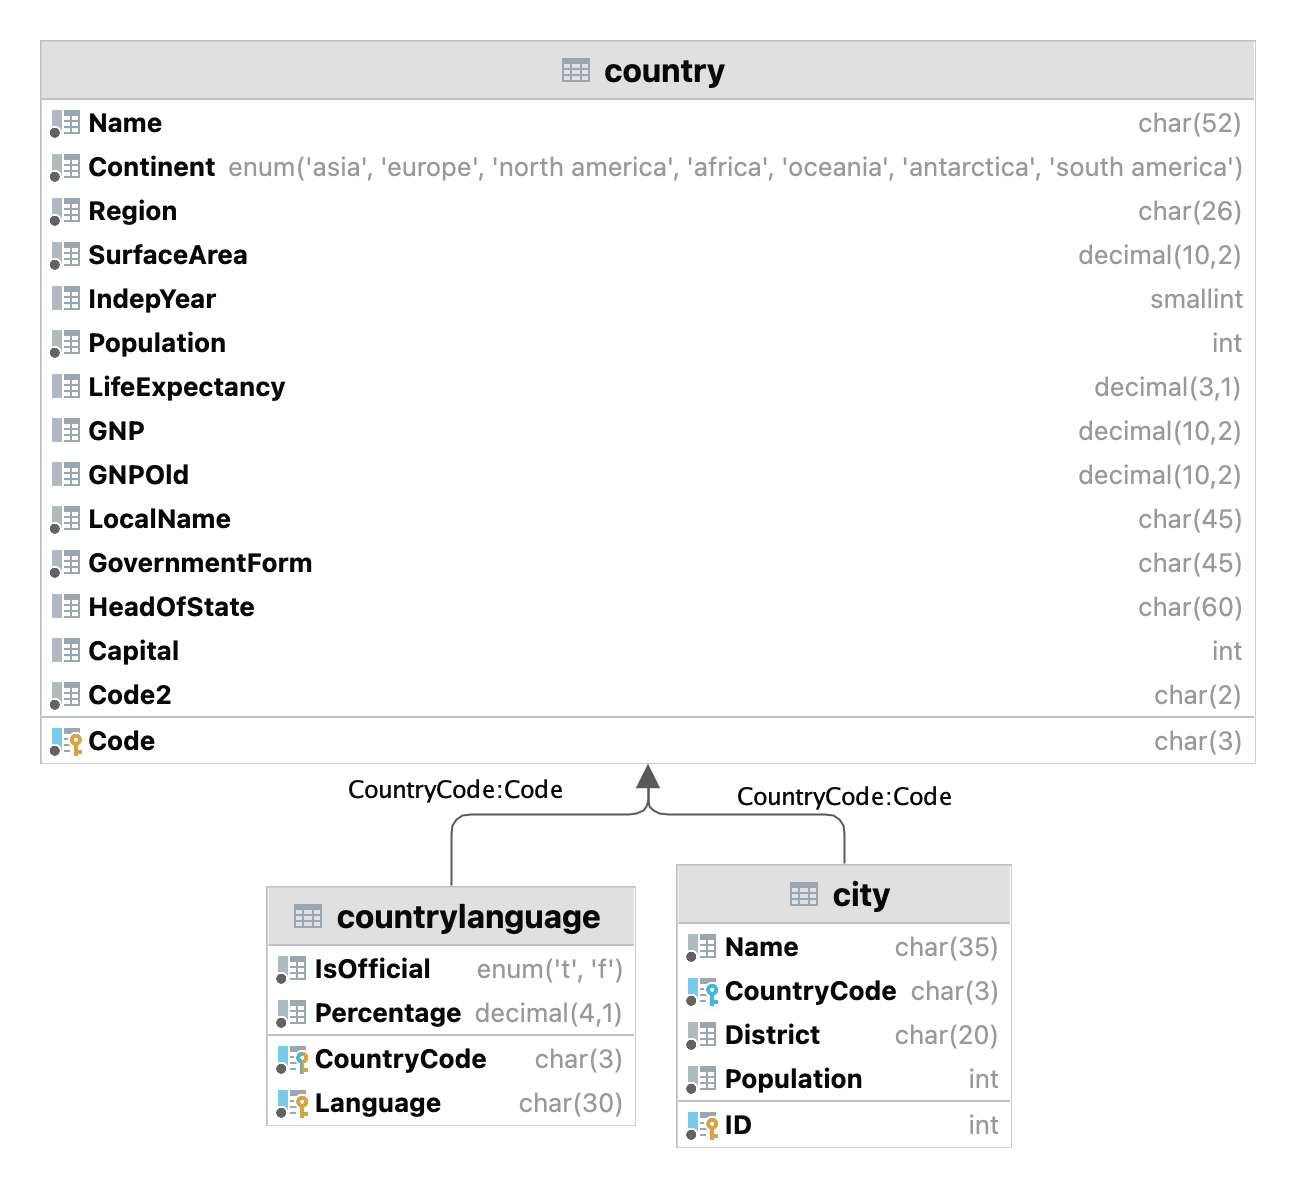
\includegraphics[scale=0.25]{capitoli/immagini/17_world_database.png}
    \caption{Diagramma del Database World}
    \label{fig:database}
\end{figure}

\subsection{Modifiche}
Una volta importato il progetto i cambiamenti da effettuare lato codice sono semplici. Prima di tutto dobbiamo dichiarare una nuova dipendenza. L'applicazione era stata creata per esporre delle API, non era previsto il suo ingresso in un'applicazione basata sui microservizi, quindi nel pom andremmo ad aggiungere la dipendenza per poter far si che il servizio possa essere scoperto da Eureka:

\begin{lstlisting}[language=xml, caption= Dipendenza di Eureka Client]
<dependency>
    <groupId>org.springframework.cloud</groupId>
    <artifactId>spring-cloud-starter-netflix-eureka-client</artifactId>
    <version>3.1.4</version>
</dependency>
\end{lstlisting}

Nel file di configurazione dobbiamo dare un nome al nostro servizio per poter essere registrato, una porta diversa dalla configurazione di base di Spring Boot (la porta 8080) e infine dobbiamo specificare l'URL del servizio di discovery Eureka:
\begin{lstlisting}[caption = Configurazione per Eureka]
#Eureka Client
spring.application.name=WORLD-SERVICE

server.port=8000
eureka.client.service-url.default-zone=http://localhost:8761/eureka
\end{lstlisting}

L'ultima modifica che dobbiamo effettuare è al file di configurazione del servizio che offre il Gateway. Questo perché, come visto in precedenza il gateway deve poter riconoscere l'instradamento dei servizi, quindi non ci resta che aggiungere il percorso per il nostro nuovo servizio:

\begin{lstlisting}[caption= Configurazione per il Gateway]
spring.cloud.gateway.routes[2].id=world
spring.cloud.gateway.routes[2].uri=lb://WORLD-SERVICE
spring.cloud.gateway.routes[2].predicates[0]=Path=/api/**
\end{lstlisting}

Una volta effettuato il deploy di tutti i servizi, possiamo notare sulla dashboard di Eureka che il nostro servizio è attivo ed è stato registrato:

\begin{figure}[h]
    \centering
    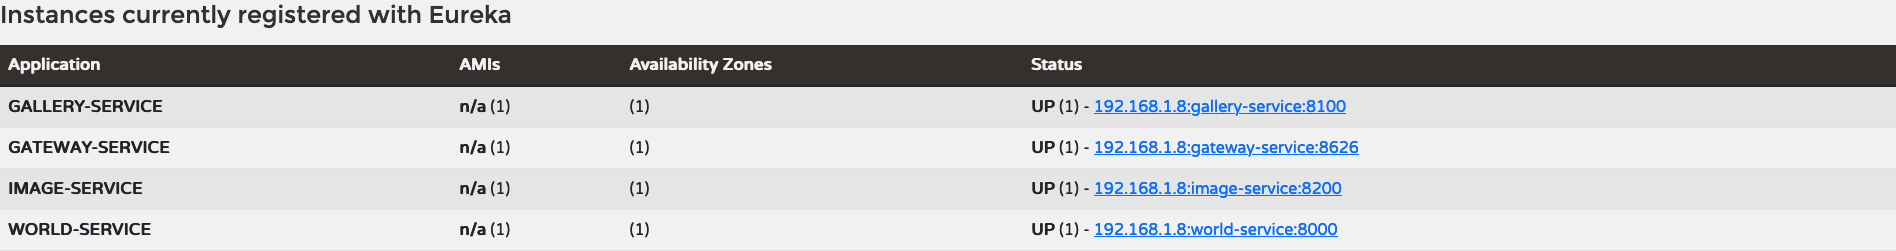
\includegraphics[scale = 0.20]{capitoli/immagini/18_world_eureka.png}
    \caption{World Service è registrato su Eureka}
    \label{fig:world_eureka}
\end{figure}